\documentclass[journal]{IEEEtran}
\usepackage[T1]{fontenc}
\usepackage{cite}
\usepackage{amsmath,amssymb}
\usepackage{graphicx}
\usepackage{booktabs}
\usepackage{multirow}
\usepackage{xcolor}
\usepackage{url}
\usepackage{stfloats}
\usepackage{balance}

% Values that have not been measured yet are printed in red so they cannot be mistaken for results.
\newcommand{\pending}[1]{\textcolor{red}{[#1]}}

\hyphenation{micro-service micro-services Kuber-netes Log-BERT Deep-Log}

\begin{document}

\title{Proactive Microservice Failure Mitigation using LogBERT Anomaly Detection in Kubernetes}

\author{Akella~Harshith~Saipaavan,
        Bavikadi~Mohaseen~Hussain,
        M~Jaidev,
        and~Ponna~Manish~Reddy%
\thanks{The authors are with the Department of Information Technology, Chaitanya Bharathi Institute of Technology (A), Hyderabad 500075, India (roll nos. 160124737166, 160124737170, 160124737186 and 160124737192).}}

\markboth{Manuscript draft}{Saipaavan \MakeLowercase{\textit{et al.}}: Proactive Microservice Failure Mitigation using LogBERT in Kubernetes}

\maketitle

\begin{abstract}
Kubernetes restarts a container once its liveness probe fails and adds replicas once average CPU use crosses a target, so it reacts only after a fault is visible to users. Container logs often show the fault earlier, and learned log anomaly detectors report high accuracy on archived benchmarks. It is less clear whether they beat simple rules on live microservice logs, and whether their verdicts are reliable enough to act on. We study both questions with a closed-loop system that parses the logs of every service into template sequences, scores sliding windows with LogBERT and passes persistent anomalies to a rule-based controller that restarts or scales the affected Deployment through the Kubernetes API, under a cool-down and an action budget. On a single-node Minikube cluster running Online Boutique we injected pod kills, scale-to-zero outages and CPU throttling, fixed every threshold on one fault run and used a second only for evaluation. LogBERT reaches a window-level F1-score of 0.912 (precision 0.970, recall 0.861). DeepLog and a keyword rule both reach 0.897, and Isolation Forest 0.419. All sequence models detect pod kills and outages well but fall to 0.58--0.61 on CPU throttling, whose symptoms lie in timing rather than message order, and removing LogBERT's hypersphere objective, service embedding or half of its layers does not lower its score. On this application, then, a learned detector adds little for faults that produce explicit errors and is not yet enough for faults that do not. Counted per episode, LogBERT flags all 18 test faults within a median of 2.3--4.5\,s of injection, but for pod kills and outages its first verdict coincides with the first failed user request, so the logs give no early warning for these faults. In a paired closed-loop run the controller recovered faster than plain Kubernetes where both let requests fail (41.8\,s against 97.4\,s over four episodes), but availability did not improve (92.4\% against 92.1\%), because the controller's restarts of the frontend caused failures of their own and 4.5 actions per hour were unnecessary. The testbed and labelling protocol are released so that the comparison can be repeated on other applications.
\end{abstract}

\begin{IEEEkeywords}
AIOps, anomaly detection, fault injection, Kubernetes, log analysis, LogBERT, microservices, self-healing systems.
\end{IEEEkeywords}

\section{Introduction}
\IEEEPARstart{A}{n} application built from microservices is a set of small programs that call each other over the network~\cite{dragoni2017}. Each service can be deployed and scaled on its own, which is why the style has spread, but the number of ways the whole system can fail grows with every service and every call between them. A cart service that loses its cache, a catalogue service that runs out of CPU or a single pod caught in a crash loop can stall the checkout path that users see.

Kubernetes~\cite{burns2016} gives such applications basic self-repair. The kubelet restarts a container whose liveness probe stops answering, and the Horizontal Pod Autoscaler (HPA) adds replicas when the average CPU use of a Deployment crosses a target. Both mechanisms are reactive. A probe fails only after the container is already unresponsive, and an average over a metrics window moves only after the load has built up. Some faults are not covered at all: when a Deployment is scaled to zero by mistake, no probe runs and the HPA has nothing to measure.

Logs are a cheaper and often earlier signal. A healthy service writes a small, repetitive set of messages; a failing one writes timeouts, refused connections, retries and stack traces, and its callers start logging errors about it. Learned log anomaly detectors such as DeepLog~\cite{du2017} and LogBERT~\cite{guo2021} model the order of these messages and report high accuracy on public benchmarks~\cite{he2016,zhu2023}. Most of that work stops at the detection score, however, and evaluates on archived logs from systems such as HDFS or supercomputers. Whether the score is good enough to act on automatically, inside the orchestrator that runs the services, is a separate question that existing studies rarely test~\cite{notaro2021,soldani2022}.

We therefore ask three questions.
\begin{itemize}
\item \textbf{RQ1:} On live microservice logs, does a learned sequence model detect injected faults better than simple baselines, including a keyword rule?
\item \textbf{RQ2:} Which faults leave too little trace in the logs, and which parts of LogBERT matter?
\item \textbf{RQ3:} Does acting on log anomalies shorten recovery compared with the mechanisms Kubernetes already has?
\end{itemize}

We answer them on a small, reproducible testbed. Our contributions are as follows.
\begin{enumerate}
\item A closed-loop system that collects container logs through the Kubernetes API, parses them with Drain~\cite{he2017}, scores per-service windows with LogBERT and maps persistent anomalies to restart or scale actions under a cool-down and an action budget (Section~\ref{sec:arch}).
\item An evaluation protocol for live microservice logs: faults injected through the Kubernetes API, labels that follow the service call graph, an exclusion period after each fault, a separate validation run for every threshold and a prober that defines what a user-visible failure is (Section~\ref{sec:setup}).
\item Evidence that, on this application, a keyword rule matches LogBERT and DeepLog on faults that produce explicit errors, that all sequence models miss much of a CPU-throttling fault, and that LogBERT's additional components bring no measurable gain, together with a comparison of closed-loop recovery against Kubernetes' built-in mechanisms (Sections~\ref{sec:results} and~\ref{sec:disc}).
\end{enumerate}

\section{Related Work}
\subsection{Log-Based Anomaly Detection}
Early detectors counted log events per window and applied PCA, invariant mining or clustering; He~\textit{et al.}~\cite{he2016} compared these methods on HDFS and BGL. DeepLog~\cite{du2017} replaced counting with an LSTM that predicts the next log key and flags a window when the observed key is not among the $g$ most likely ones. LogAnomaly~\cite{meng2019} added template semantics so that new but similar messages are not treated as anomalies, and LogRobust~\cite{zhang2019} used attention over semantic vectors to cope with logs that change between releases. LogBERT~\cite{guo2021} applies a bidirectional Transformer encoder~\cite{vaswani2017,devlin2019} trained to predict masked log keys, together with a hypersphere objective adapted from Deep SVDD~\cite{ruff2018}, and reported better F1-scores than DeepLog and LogAnomaly on HDFS, BGL and Thunderbird. NeuralLog~\cite{le2021} skips parsing and feeds raw messages to a Transformer. Le and Zhang~\cite{le2022} later showed that reported results depend strongly on how the data are split, on label noise and on parsing quality, which is one reason we keep a strict separation between validation and test runs.

\subsection{Log Parsing}
All key-based detectors depend on a parser that turns free-text messages into templates. Drain~\cite{he2017} builds a fixed-depth tree over message tokens, runs online and was among the most accurate parsers in the benchmark of Zhu~\textit{et al.}~\cite{zhu2019}. The Loghub collection~\cite{zhu2023} provides the datasets on which most parsers and detectors are compared.

\subsection{Large Language Models for Log Analysis}
Since 2023 large language models have been applied to both parsing and detection. LogPPT~\cite{le2023} parses logs by few-shot prompting of a pretrained model, and LILAC~\cite{jiang2024} adds a parsing cache so that repeated messages do not trigger new queries. LogGPT~\cite{han2023}, from the group that proposed LogBERT, trains a GPT-style model to predict the next log key and fine-tunes it with reinforcement learning. These models are far larger and slower per window than the 3.2\,M-parameter encoder used here. We keep a small model because the detector has to score every window of every service in real time on a laptop GPU, and leave a comparison with LLM-based detectors to future work.

\subsection{Failure Management for Microservices}
Surveys of AIOps~\cite{notaro2021} and of anomaly detection and root-cause analysis for microservices~\cite{soldani2022} show that most methods work on metrics or traces, and that remediation is studied far less than detection. Root-cause methods such as MicroRCA~\cite{wu2020} rank suspect services from metric anomalies on the call graph. Benchmark applications such as DeathStarBench~\cite{gan2019} and TrainTicket~\cite{zhou2021} and the Online Boutique demo~\cite{onlineboutique} make such studies repeatable, and chaos engineering~\cite{basiri2016} supplies the fault injection. Our controller follows the monitor--analyse--plan--execute loop of autonomic computing~\cite{kephart2003}, with logs as the monitored signal and the Kubernetes API as the effector.

Closer to our goal, Seer~\cite{gan2019seer} trains a deep network on distributed traces to predict quality-of-service violations in microservices before they happen and signals the cluster manager to adjust resources, and FIRM~\cite{qiu2020} uses reinforcement learning to reprovision the microservices responsible for service-level-objective violations. Both act on traces and performance counters rather than logs. At the level of whole incidents, Ahmed~\textit{et al.}~\cite{ahmed2023} use large language models to recommend root causes and mitigation steps, and RCACopilot~\cite{chen2024} collects diagnostic data and predicts the root-cause category with an LLM; in both, engineers still carry out the mitigation.

\section{System Architecture}\label{sec:arch}
Fig.~\ref{fig:arch} shows the system. All components except the services themselves run as processes on the host and talk to the cluster only through the Kubernetes API, so the application does not have to be changed.

\begin{figure*}[!t]
\centering
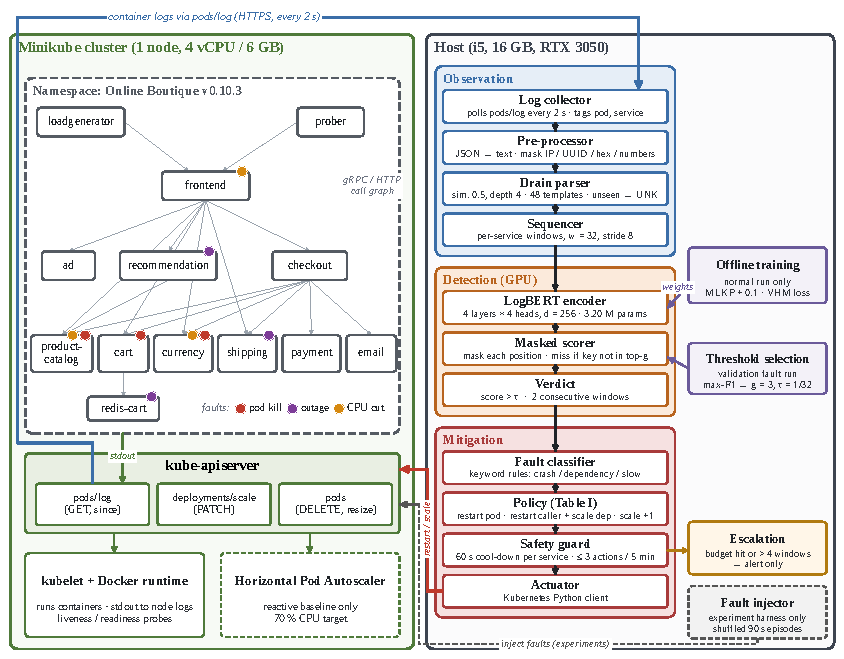
\includegraphics[width=\textwidth]{fig1_architecture.pdf}
\caption{System architecture. Left: the single-node Minikube cluster running Online Boutique; grey arrows are service calls and coloured dots mark the services targeted by each fault type. Right: the host-side pipeline. Blue: log flow from the API server to the collector. Red: mitigation actions. Dashed: paths used only during training and experiments.}
\label{fig:arch}
\end{figure*}

\subsection{Log Collection and Parsing}
The collector polls the \texttt{pods/log} endpoint of every monitored pod every 2\,s, asks only for lines newer than the last poll and tags each line with its pod and service. Online Boutique services write JSON; the pre-processor keeps the severity, the message and the class of any HTTP status code and drops the rest. Numbers, IP addresses, UUIDs and hexadecimal identifiers are then replaced by placeholders, and the service name is prefixed to the line so that the same message from two services yields two different keys.

Drain runs with a similarity threshold of 0.5 and a tree depth of 4. Templates are learned from the normal run only, which gives 48 templates. A message that matches no template at run time is mapped to a reserved unknown key instead of creating a new template, so the vocabulary of the detector stays fixed. The sequencer keeps a buffer per service and emits a window of $w = 32$ consecutive keys every 8 keys.

\subsection{LogBERT Detector}
Fig.~\ref{fig:logbert} shows the detector. Each key in a window is embedded and added to a positional embedding and to an embedding of the service that produced the window. A Transformer encoder with 4 layers, 4 attention heads and a hidden size of 256 (3.20\,M parameters) processes the window in both directions.

\begin{figure*}[!t]
\centering
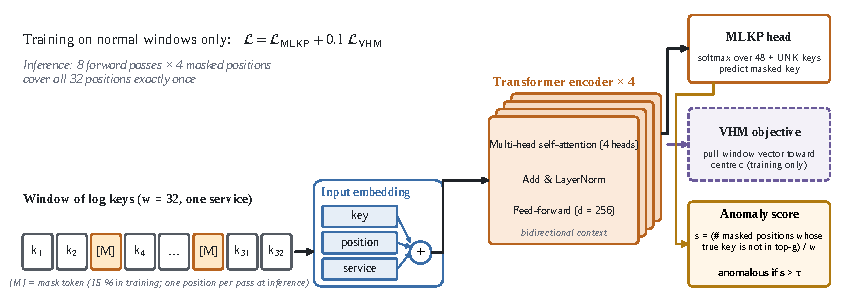
\includegraphics[width=0.91\textwidth]{fig2_logbert.pdf}
\caption{LogBERT detector. Keys, positions and the service identity are embedded and summed, encoded by four Transformer layers and passed to a masked-key prediction head. The hypersphere (VHM) objective is used only in training. At inference every position is masked once and the anomaly score is the share of positions whose true key is not among the top-$g$ predictions.}
\label{fig:logbert}
\end{figure*}

Training uses normal windows only and combines two self-supervised losses. In masked log-key prediction (MLKP), 15\% of the positions are replaced by a mask token and the model predicts the original key from the context on both sides. The volume-of-hypersphere loss (VHM) pulls the pooled representation of each normal window towards a fixed centre $\mathbf{c}$, as in Deep SVDD~\cite{ruff2018}. The total loss is
\begin{equation}
\mathcal{L} = \mathcal{L}_{\mathrm{MLKP}} + 0.1\,\mathcal{L}_{\mathrm{VHM}}.
\end{equation}
We train with AdamW (learning rate $10^{-3}$, batch size 256, seed 0) for 40 epochs. The held-out loss stops improving after about 20 epochs while the training loss keeps falling, a sign of mild overfitting; we did not use early stopping.

At inference each of the 32 positions is masked exactly once, in 8 forward passes of 4 masked positions. A position is a miss when its true key is not among the $g$ most probable keys, and the anomaly score of a window is
\begin{equation}
s = \frac{\text{number of misses}}{w}.
\end{equation}
A window is anomalous when $s > \tau$. Both $g$ and $\tau$ are chosen on the validation run by maximising the F1-score, which gives $g = 3$ and $\tau = 1/32 \approx 0.031$. The comparison is strict and $\tau$ equals the score of a window with exactly one miss, so a window is flagged only when at least two of its 32 keys are missed. Under normal load the log stream of each service is regular enough that the model rarely misses twice in one window.

\subsection{Mitigation Controller}
The controller (Fig.~\ref{fig:controller}) acts on a service only after two consecutive anomalous windows from that service, which filters isolated spikes. It then assigns a coarse fault class from keywords in the raw lines of the anomalous window. Timeouts, refused connections and RPC errors mark a dependency fault, and any other service named in those lines is taken as the failing dependency. Panics, exceptions and out-of-memory messages mark a crash. A window with neither is treated as a slow handler. Table~\ref{tab:policy} maps each class to the least disruptive action we could think of for it.

\begin{figure}[!t]
\centering
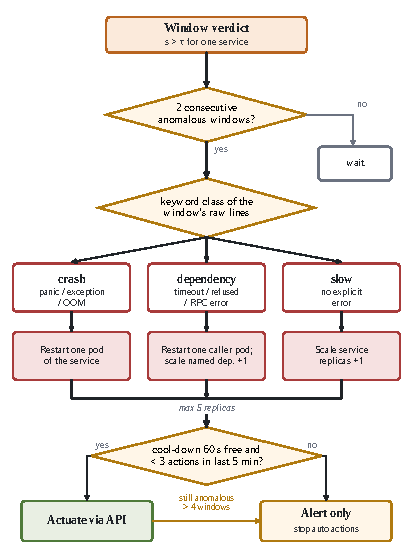
\includegraphics[width=\columnwidth]{fig3_controller.pdf}
\caption{Decision flow of the mitigation controller.}
\label{fig:controller}
\end{figure}

\begin{table}[!t]
\centering
\caption{Mitigation Policy}
\label{tab:policy}
\setlength{\tabcolsep}{4pt}
\begin{tabular}{@{}p{2.55cm}p{5.6cm}@{}}
\toprule
Suspected fault & Action \\
\midrule
Crash or exception burst & Restart one pod of the service \\
Dependency error & Restart one caller pod; scale each named dependency by $+1$ (max.\ 5 replicas) \\
No explicit error (slow handler) & Scale the service by $+1$ (max.\ 5 replicas) \\
Still anomalous for $>4$ windows after an action & Alert only; stop automatic actions for the service \\
\bottomrule
\end{tabular}
\end{table}

Two guards limit the damage a wrong verdict can do. Each service has a cool-down of 60\,s between actions, and the controller as a whole may take at most three automatic actions in any five minutes; beyond that it only raises an alert. A restart deletes one pod at a time, so a Deployment with several replicas never loses all of them at once. The actuator uses the official Kubernetes Python client and needs only the permissions to delete pods and patch the scale of Deployments.

\section{Experimental Setup}\label{sec:setup}
\subsection{Testbed}
All experiments run on one laptop (Intel Core i5, 16\,GB RAM, NVIDIA RTX 3050 with 6\,GB, Windows~11). Minikube 1.39 with the Docker driver hosts a single-node cluster running Kubernetes v1.37.0, limited to 4 vCPU and 6\,GB of memory. The cluster runs release v0.10.3 of Online Boutique~\cite{onlineboutique}, which has 11 services written in Go, C\#, Node.js, Python and Java plus a Redis cache; 10 services are monitored. Load comes from the bundled load generator with its default 10 simulated users. A separate prober pod requests the home page, a product page and the cart in a loop with a 0.5\,s pause and a 3\,s timeout. A failed probe is our definition of a user-visible failure. LogBERT is trained and run on the laptop GPU; Table~\ref{tab:params} lists the settings.

\begin{table}[!t]
\centering
\caption{Implementation Settings}
\label{tab:params}
\begin{tabular}{@{}ll@{}}
\toprule
Setting & Value \\
\midrule
Log polling interval & 2\,s \\
Drain similarity / depth & 0.5 / 4 \\
Templates (incl.\ service prefix) & 48 \\
Window size / stride & 32 / 8 keys \\
Encoder layers / heads / hidden size & 4 / 4 / 256 \\
Parameters & 3.20\,M \\
Mask ratio in training & 15\% \\
VHM weight & 0.1 \\
Training epochs & 40 (about 8\,s each on the GPU) \\
Optimizer / learning rate / batch & AdamW / $10^{-3}$ / 256 \\
Top-$g$ / threshold $\tau$ & 3 / $1/32$ \\
Persistence & 2 consecutive windows \\
Cool-down / action budget & 60\,s per service / 3 per 5\,min \\
\bottomrule
\end{tabular}
\end{table}

\subsection{Fault Injection}
Faults are injected through the Kubernetes API rather than a chaos tool, which keeps the setup to a single cluster without extra operators. Table~\ref{tab:faults} lists the three types and their targets. Each episode lasts about 90\,s, the target and fault type follow a shuffled schedule, and episodes are separated by about two minutes of normal traffic.

\begin{table}[!t]
\centering
\caption{Injected Fault Types}
\label{tab:faults}
\setlength{\tabcolsep}{3pt}
\begin{tabular}{@{}p{1.35cm}p{3.2cm}p{3.6cm}@{}}
\toprule
Fault & Mechanism & Targets \\
\midrule
Pod kill & Force-delete the running pod every 20\,s & productcatalog, currency, cart \\
Outage & Scale the Deployment to zero replicas & redis-cart, recommendation, shipping \\
CPU throttling & Cut the CPU limit of the running pod in place to 10 millicores & frontend, productcatalog, currency \\
\bottomrule
\end{tabular}
\end{table}

\subsection{Dataset and Labelling}
Fig.~\ref{fig:protocol} shows the protocol. The normal run contains no faults and is used to learn the Drain templates and to train every detector. It is not error-free: the load generator occasionally triggers a failed checkout or ad lookup, and those lines are kept so that the detectors learn them as normal. Two fault runs of 18 episodes each follow, one for validation and one for test, with different schedules. Each run covers every fault--target pair twice.

\begin{figure*}[!t]
\centering
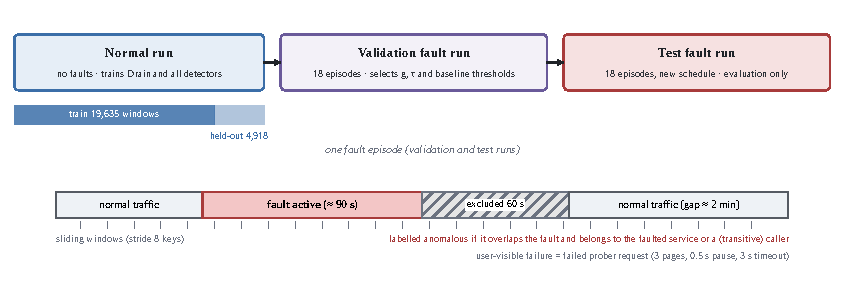
\includegraphics[width=\textwidth]{fig4_protocol.pdf}
\caption{Experimental protocol. The normal run trains all detectors; the validation run fixes every threshold; the test run is used only for evaluation. Bottom: labelling within one fault episode.}
\label{fig:protocol}
\end{figure*}

A window is labelled anomalous if it overlaps an injected interval and comes from the faulted service or from a service that calls it, directly or through other services, according to the static call graph of Online Boutique. Windows that start within 60\,s after a fault ends are excluded from scoring, because the application is still recovering and neither label is clearly right. The normal run lasts 44.6\,min and is split by time: windows from the first 32\,min train LogBERT, windows from the last 12.5\,min are held out, and the 37 windows that straddle the cut are dropped. The 196,999 normal lines in Table~\ref{tab:data} are those of the 10 monitored services; the load generator and the prober wrote another 35,458 lines that no detector sees. Consecutive windows share 24 of their 32 keys, so window-level counts are not independent samples; we therefore also report detection per fault episode (Section~\ref{sec:episodes}). Table~\ref{tab:data} summarises the data.

\begin{table}[!t]
\centering
\caption{Dataset Summary}
\label{tab:data}
\begin{tabular}{@{}lr@{}}
\toprule
Item & Value \\
\midrule
Monitored services / templates & 10 / 48 \\
Normal log lines & 196,999 \\
Training / held-out windows (normal run) & 19,635 / 4,918 \\
Validation windows (normal / anomalous) & 21,557 / 6,640 \\
Test windows (normal / anomalous) & 21,900 / 6,443 \\
Fault episodes (validation / test) & 18 / 18 \\
\bottomrule
\end{tabular}
\end{table}

\subsection{Baselines and Metrics}
We compare LogBERT with three detectors. The keyword rule flags a window when any of its lines contains \emph{error}, \emph{fail}, \emph{exception}, \emph{fatal}, \emph{panic}, \emph{timeout}, \emph{timed out}, \emph{refused} or \emph{unavailable}, ignoring case. Isolation Forest~\cite{liu2008} uses 100 trees on template-count vectors. DeepLog~\cite{du2017} is a two-layer LSTM (embedding size 64, hidden size 128) that predicts each key from the previous 10, trained with Adam (learning rate $10^{-3}$, batch size 1024) for 5 epochs; its validation-selected settings are $g = 2$ and a window threshold of 0.091. Both learned baselines are fitted on all 24,590 normal windows, including the part held out from LogBERT, which slightly favours them. Every threshold is chosen on the validation run and frozen for the test run. During development the evaluation script read the test run three times, always with the same models and thresholds and with identical results; nothing was tuned on it.

The mitigation baseline is plain Kubernetes: the liveness and readiness probes shipped with Online Boutique, plus an HPA with a 70\% CPU target on the services that receive the CPU-throttling fault. For detection we report window-level precision, recall and F1-score. For mitigation we report the detection lead time (from the first verdict on an affected service to the first failed probe, positive when the verdict comes first), the mean time to recovery (MTTR, from the first failed probe to the start of the first 10\,s without a failed probe) and availability (the share of successful probes). Each condition is measured in a single run.

The recovery comparison uses pod kill and CPU throttling only. A Deployment scaled to zero cannot be recovered by probes or the HPA until the fault is withdrawn, whereas the controller's scale action reverses it directly; including the outage fault in the main comparison would favour the controller by construction, so we report it separately. Pod kill is not biased in the same way, but Kubernetes already recreates a deleted pod by itself. For this fault a restart of the same pod gains nothing, so the comparison mainly tests whether the controller's actions on callers and dependencies help or interfere with the built-in recovery.

\section{Results}\label{sec:results}
\subsection{Detection Quality}
Table~\ref{tab:detect} gives the test results. LogBERT has the highest F1-score, 0.912, but DeepLog and the keyword rule (both 0.897) are only 0.015 behind. With one run per method we do not treat that gap as meaningful. The methods differ more in how they err: the keyword rule has a precision of 0.997 but misses 18.5\% of the anomalous windows, while LogBERT gives up 2.7 points of precision for 4.6 points of recall. Isolation Forest on template counts is far behind (0.419), with most of its alarms false. Count vectors discard the order of messages, and a likely reason is that ordinary changes in traffic volume move them about as much as a fault does.

\begin{table}[!t]
\centering
\caption{Detection Results on the Test Run}
\label{tab:detect}
\begin{tabular}{@{}lccc@{}}
\toprule
Method & Precision & Recall & F1 \\
\midrule
Keyword rule & \textbf{0.997} & 0.815 & 0.897 \\
Isolation Forest & 0.324 & 0.591 & 0.419 \\
DeepLog & 0.943 & 0.855 & 0.897 \\
LogBERT & 0.970 & \textbf{0.861} & \textbf{0.912} \\
\bottomrule
\end{tabular}

\end{table}

Fig.~\ref{fig:perfault} splits the F1-score by fault type. Pod kills and outages are loud: the affected service stops logging and its callers start logging refused connections and RPC errors, so LogBERT reaches 0.93 on both and DeepLog 0.89--0.91. CPU throttling is quiet. A throttled service keeps writing the same messages, only more slowly, and its callers log errors only when their requests time out. LogBERT falls to 0.612 and DeepLog to 0.577 on this fault. A model that sees only the order of keys cannot see that they have slowed down; adding inter-arrival times to the input is the most direct fix.

\begin{figure}[!t]
\centering
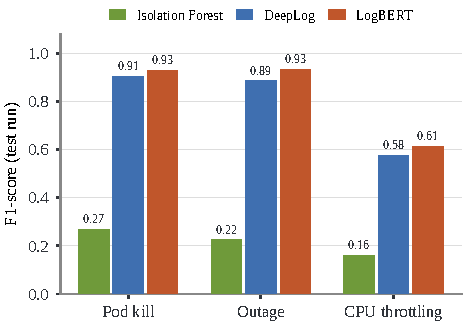
\includegraphics[width=\columnwidth]{fig5_f1_per_fault.pdf}
\caption{F1-score per fault type on the test run, computed on the windows of that fault together with all normal windows.}
\label{fig:perfault}
\end{figure}

Fig.~\ref{fig:threshold} shows how the LogBERT result on the test run moves with the threshold. Precision is already above 0.99 at $\tau = 0.1$ and stays there, while recall falls steadily, so every threshold above the validation choice gives up recall for almost no gain in precision. The F1-score on the test run peaks near $\tau = 0.05$, close to the value selected on the validation run. The test F1-score at the chosen threshold, 0.91, is within about 0.01 of the best point on the curve, so fixing $\tau$ on a separate run cost almost nothing here.

\begin{figure}[!t]
\centering
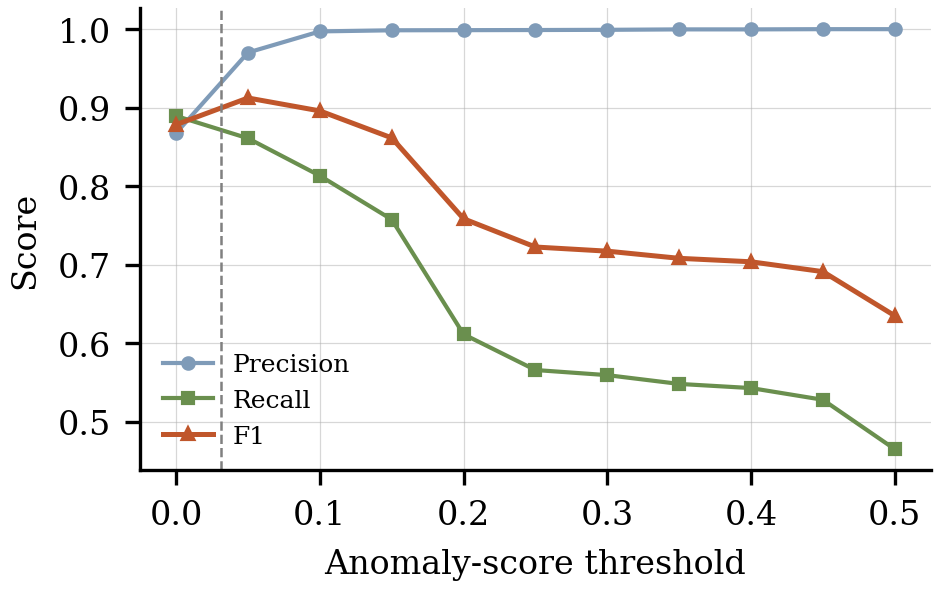
\includegraphics[width=\columnwidth]{fig6_threshold.png}
\caption{Precision, recall and F1-score of LogBERT on the test run as a function of the anomaly-score threshold. The dashed line marks the value chosen on the validation run, $\tau = 1/32$.}
\label{fig:threshold}
\end{figure}

\subsection{Episode-Level Detection}\label{sec:episodes}
Window-level scores give long episodes more weight and count overlapping windows separately. Table~\ref{tab:episodes} therefore reports, for each fault type, how many of the six test episodes produced at least one verdict on an affected service and how long after injection LogBERT's first verdict came. The numbers come from replaying the stored window scores offline, not from the live controller. DeepLog's trained model was not kept, so it is omitted here.

\begin{table}[!t]
\centering
\caption{Episode-Level Detection on the Test Run (Offline Replay)}
\label{tab:episodes}
\setlength{\tabcolsep}{4pt}
\begin{tabular}{@{}lccc@{}}
\toprule
& \multicolumn{2}{c}{Episodes detected (of 6)} & LogBERT median time \\
\cmidrule(lr){2-3}
Fault & LogBERT & Keyword rule & to first verdict (s) \\
\midrule
Pod kill & 6 & 6 & 2.3 \\
Outage & 6 & 6 & 3.9 \\
CPU throttling & 6 & 5 & 4.5 \\
\midrule
Total & 18 & 17 & -- \\
\bottomrule
\end{tabular}
\end{table}

LogBERT detects all 18 episodes and the keyword rule 17. Two observations temper these counts. First, the verdicts are not early warnings. For pod kill and outage, LogBERT's first verdict arrives at the same moment as the first failed probe; only CPU throttling shows a lead, of 2.4 to 23.0\,s in four of its six episodes. Second, LogBERT also produced 89 false verdict windows during the 1.13\,h of normal traffic in the test run. With 90\,s episodes, some detections could therefore be chance, most plausibly the two throttling episodes in which no probe failed at all.

\subsection{Ablation}
Table~\ref{tab:ablation} changes one component at a time. None of the three changes to the model lowers the F1-score; removing the VHM objective, removing the service embedding or halving the encoder gives an F1-score of 0.916--0.917, with higher precision and slightly lower recall. With only 48 templates and highly regular normal traffic, masked-key prediction by a small encoder already captures what there is to learn, and the additional components bring no measurable benefit on this application. The last row applies the controller's two-window persistence rule to the full model's window verdicts: precision rises to 0.984 and recall falls to 0.843 (F1-score 0.908), which is the trade the controller accepts to avoid acting on single windows.

\begin{table}[!t]
\centering
\caption{Ablation on the Test Run}
\label{tab:ablation}
\begin{tabular}{@{}lccc@{}}
\toprule
Variant & Precision & Recall & F1 \\
\midrule
Full model & 0.970 & 0.861 & 0.912 \\
Without VHM objective & 0.986 & 0.858 & 0.917 \\
Without service embedding & 0.983 & 0.858 & 0.916 \\
Encoder with 2 layers & 0.985 & 0.858 & 0.917 \\
Full model + 2-window persistence & 0.984 & 0.843 & 0.908 \\
\bottomrule
\end{tabular}

\end{table}

\subsection{Early Warning and Recovery}
We ran one new schedule of 18 episodes, used by neither the validation nor the test run, twice: once with plain Kubernetes and once with the controller. In the reactive run the detector ran in observe-only mode, so its verdict times were recorded but no action was taken. In both runs every Deployment was set back to one replica 60\,s after each episode. Table~\ref{tab:loop} summarises pod kill and CPU throttling.

\begin{table}[!t]
\centering
\caption{Mitigation Outcomes on Pod Kill and CPU Throttling (12 Episodes, One Run Each)}
\label{tab:loop}
\begin{tabular}{@{}lcc@{}}
\toprule
Metric & Reactive & Controller \\
\midrule
Mean time to recovery (s) & 97.4 & 32.2 \\
\quad over episodes with failed probes & 4 & 10 \\
Availability (\%) & 92.07 & 92.43 \\
Failed probes during faults (\%) & 12.6 & 11.0 \\
Episodes not recovered before fault end & 0 & 0 \\
Automatic actions, whole run & -- & 36 \\
Unnecessary actions per hour & -- & 4.5 \\
Median detection lead time (s) & 0.1\textsuperscript{a} & 0.0 \\
\bottomrule
\end{tabular}

\smallskip
\footnotesize\textsuperscript{a}Detector in observe-only mode.
\end{table}

The means in Table~\ref{tab:loop} are taken over different episodes, because the two runs failed in different places. In the four episodes in which both runs had failed probes, the controller recovered faster in every case, with a mean of 41.8\,s against 97.4\,s; the clearest cases are the two cart-service kills (86.5 and 28.0\,s against 137.5 and 124.9\,s). In six further episodes only the controller run had failed probes. In five of them the loss was small (2.3--4.5\% of probes), and in one currency-service kill it was 40.7\%. Two effects explain the difference. First, after the frontend was throttled in the fifth episode of the reactive run, the HPA scaled the frontend to four or five replicas and kept them, overriding the reset, so later faults met a better-provisioned frontend than in the controller run, which had no HPA. The test run, which had neither, lost 66--73\% of probes to the same currency-service kill. Second, the controller restarted a frontend pod 11 times; the frontend starts every episode with one replica, and a restart of the only replica drops requests until its replacement is ready. As a result availability is practically the same in both runs (92.43\% against 92.07\%), and the faster recovery when both runs fail is offset by failures that the controller does not prevent or causes itself. It also took 4.5 unnecessary actions per hour.

The controller did not act early either. With the detector observing only, its median lead over the first failed probe was 0.1\,s; with the controller acting it was 0.0\,s. As in the offline replay, only CPU throttling gave a real lead, with a median of 19.1\,s over the two throttling episodes of the reactive run that had failed probes.

For the outage fault, reported separately for the reason given in Section~\ref{sec:setup}, the MTTR is 73.4\,s for the baseline and 56.1\,s for the controller, with 11.9\% and 18.5\% of probes failing during the fault. The controller ended one shipping-service outage after 39.9\,s instead of 125.6\,s, but it made both Redis outages worse (55.2\% and 21.5\% of probes failed against 9.1\% and 9.0\%), because it restarted callers that could not recover while the cache was still down.

\section{Discussion}\label{sec:disc}
\subsection{Answers to the Research Questions}
\textbf{RQ1.} Not measurably, at window level. LogBERT has the highest F1-score, but DeepLog and the keyword rule are 0.015 behind it in a single run; LogBERT finds more anomalous windows than the rule at the cost of some false alarms. Per episode, LogBERT detects all 18 test faults and the rule 17.

\textbf{RQ2.} CPU throttling is the fault the logs barely show: LogBERT and DeepLog fall to 0.61 and 0.58 on it. None of LogBERT's additions to a plain masked-key encoder (the hypersphere objective, the service embedding, the extra layers) improved the result on this 48-template vocabulary.

\textbf{RQ3.} Not in this testbed. When both the controller and plain Kubernetes let requests fail, the controller recovers faster (41.8\,s against 97.4\,s over four paired episodes), but availability over pod kill and CPU throttling is unchanged (92.43\% against 92.07\%). Its restarts of the frontend cause failures of their own, it takes 4.5 unnecessary actions per hour, and its verdicts arrive no earlier than the first failed request. One run per condition and the HPA's lasting scale-up in the reactive run leave this answer open to revision.

\subsection{How Proactive Can Log-Based Mitigation Be?}
The episode results limit what ``proactive'' can mean on this testbed. A pod kill or an outage breaks requests at once, and the logs report the failure as it happens, so a log-based controller cannot act before users are affected; it can only act sooner and on a better target than probes and autoscaling. Early warning appeared only for CPU throttling, where performance degrades gradually and LogBERT's first verdict preceded the first failed probe by up to 23\,s. Proactive mitigation from logs is therefore most promising for gradual faults such as resource exhaustion or slow dependencies, which are also the faults that sequence models currently detect worst.

\subsection{When Is a Learned Detector Worth It?}
On Online Boutique, a keyword rule matches LogBERT on window-level F1 with almost no false alarms. That is not a weakness of the experiment but a property of the faults: pod kills and outages make services log explicit errors. The learned detectors earn their cost in two places. First, they need no list of error words, so they carry over to services whose messages the operator has never read. Second, they react to changes in the order of normal messages, which is the only symptom a quiet fault may leave. Our CPU-throttling results show that the second advantage is still limited when the symptom is in timing rather than order. A practical deployment could run the cheap rule and the learned model side by side and act when either fires.

\subsection{Threats to Validity}
The study uses one demo application, synthetic faults and a single-node cluster on a laptop. Production logs are noisier, change with every release~\cite{zhang2019} and arrive at much higher volume. Only three fault types are covered, so memory leaks and network faults are not evaluated. Each condition is a single run, so the results carry no confidence intervals and small differences between methods should not be read as rankings. Because consecutive windows overlap by 75\%, the 28,343 test windows contain far fewer independent observations than their number suggests; the 18 test episodes are the better guide to how uncertain the results are. Labels follow fault intervals and the static call graph, which blurs the exact onset and can mark a caller as anomalous even if it never noticed the fault. The fault class comes from keyword rules rather than a learned classifier, and the policy has no reschedule or resource-request action. The CPU-throttling fault lives in the running pod, so a restart removes it; a throttle caused by the workload itself would not go away that way. Logs are polled every 2\,s, which bounds how early a verdict can arrive and can lose the last lines of a container that crashes between polls. In the closed-loop comparison the HPA kept extra frontend replicas across episodes despite the reset, so the two runs did not start every episode from the same state, and the controller's dependency names come from keyword rules that we refined on the validation run. LogBERT was trained for a fixed 40 epochs although its held-out loss stopped improving after about 20, and the learned baselines saw more normal data than LogBERT did. Finally, automatic remediation can do harm when the detector is wrong, which is why the controller works under an action budget and hands persistent anomalies to a human.

\section{Conclusion}
We connected a LogBERT log anomaly detector to a guarded mitigation controller for Kubernetes and evaluated it on Online Boutique with three injected fault types. With thresholds fixed on a separate validation run, LogBERT reaches an F1-score of 0.91 on the test run, level with DeepLog and a keyword rule. It flags every test episode within a few seconds, but for pod kills and outages no earlier than the first user-visible failure, and all sequence models struggle with CPU throttling, whose symptoms are in timing rather than message order. LogBERT's hypersphere objective, service embedding and extra layers did not improve the result on this 48-template vocabulary. Acting on the verdicts shortened recovery when both the controller and plain Kubernetes let requests fail, but did not raise availability, because the controller's own restarts and unnecessary actions cost about as much as it saved; a policy that never restarts the last replica of a service is the obvious next change. Next steps are repeated runs with confidence intervals, memory and network faults, inter-arrival times as an input feature, a second application such as TrainTicket~\cite{zhou2021}, and a comparison on the public Loghub datasets~\cite{zhu2023}.

\section*{Data Availability}
The code, Kubernetes manifests, fault schedules and generated logs will be made public on publication at \pending{repository URL}.

\section*{Acknowledgment}
The authors used Claude (Anthropic), an AI assistant, to help write code, prepare figures and draft and edit the text of this manuscript. All experiments were run by the authors, every reported value comes from the authors' experiment logs, and the authors reviewed the full text and take responsibility for its content.

\balance
\begin{thebibliography}{99}

\bibitem{dragoni2017}
N.~Dragoni, S.~Giallorenzo, A.~Lluch Lafuente, M.~Mazzara, F.~Montesi, R.~Mustafin, and L.~Safina, ``Microservices: Yesterday, today, and tomorrow,'' in \emph{Present and Ulterior Software Engineering}. Cham, Switzerland: Springer, 2017, pp.~195--216.

\bibitem{burns2016}
B.~Burns, B.~Grant, D.~Oppenheimer, E.~Brewer, and J.~Wilkes, ``Borg, Omega, and Kubernetes,'' \emph{ACM Queue}, vol.~14, no.~1, 2016.

\bibitem{du2017}
M.~Du, F.~Li, G.~Zheng, and V.~Srikumar, ``DeepLog: Anomaly detection and diagnosis from system logs through deep learning,'' in \emph{Proc. ACM SIGSAC Conf. Comput. Commun. Secur. (CCS)}, 2017, pp.~1285--1298.

\bibitem{guo2021}
H.~Guo, S.~Yuan, and X.~Wu, ``LogBERT: Log anomaly detection via BERT,'' in \emph{Proc. Int. Joint Conf. Neural Netw. (IJCNN)}, 2021, pp.~1--8.

\bibitem{he2016}
S.~He, J.~Zhu, P.~He, and M.~R. Lyu, ``Experience report: System log analysis for anomaly detection,'' in \emph{Proc. IEEE 27th Int. Symp. Softw. Rel. Eng. (ISSRE)}, 2016, pp.~207--218.

\bibitem{zhu2023}
J.~Zhu, S.~He, P.~He, J.~Liu, and M.~R. Lyu, ``Loghub: A large collection of system log datasets for AI-driven log analytics,'' in \emph{Proc. IEEE 34th Int. Symp. Softw. Rel. Eng. (ISSRE)}, 2023.

\bibitem{notaro2021}
P.~Notaro, J.~Cardoso, and M.~Gerndt, ``A survey of AIOps methods for failure management,'' \emph{ACM Trans. Intell. Syst. Technol.}, vol.~12, no.~6, Art.~no.~81, 2021.

\bibitem{soldani2022}
J.~Soldani and A.~Brogi, ``Anomaly detection and failure root cause analysis in (micro)service-based cloud applications: A survey,'' \emph{ACM Comput. Surv.}, vol.~55, no.~3, Art.~no.~59, 2022.

\bibitem{he2017}
P.~He, J.~Zhu, Z.~Zheng, and M.~R. Lyu, ``Drain: An online log parsing approach with fixed depth tree,'' in \emph{Proc. IEEE Int. Conf. Web Services (ICWS)}, 2017, pp.~33--40.

\bibitem{meng2019}
W.~Meng \emph{et~al.}, ``LogAnomaly: Unsupervised detection of sequential and quantitative anomalies in unstructured logs,'' in \emph{Proc. 28th Int. Joint Conf. Artif. Intell. (IJCAI)}, 2019, pp.~4739--4745.

\bibitem{zhang2019}
X.~Zhang \emph{et~al.}, ``Robust log-based anomaly detection on unstable log data,'' in \emph{Proc. 27th ACM Joint Eur. Softw. Eng. Conf. Symp. Found. Softw. Eng. (ESEC/FSE)}, 2019, pp.~807--817.

\bibitem{vaswani2017}
A.~Vaswani \emph{et~al.}, ``Attention is all you need,'' in \emph{Proc. Adv. Neural Inf. Process. Syst. (NeurIPS)}, 2017.

\bibitem{devlin2019}
J.~Devlin, M.-W. Chang, K.~Lee, and K.~Toutanova, ``BERT: Pre-training of deep bidirectional transformers for language understanding,'' in \emph{Proc. Conf. North Amer. Chapter Assoc. Comput. Linguistics (NAACL-HLT)}, 2019, pp.~4171--4186.

\bibitem{ruff2018}
L.~Ruff \emph{et~al.}, ``Deep one-class classification,'' in \emph{Proc. 35th Int. Conf. Mach. Learn. (ICML)}, 2018, pp.~4393--4402.

\bibitem{le2021}
V.-H. Le and H.~Zhang, ``Log-based anomaly detection without log parsing,'' in \emph{Proc. 36th IEEE/ACM Int. Conf. Autom. Softw. Eng. (ASE)}, 2021, pp.~492--504.

\bibitem{le2022}
V.-H. Le and H.~Zhang, ``Log-based anomaly detection with deep learning: How far are we?'' in \emph{Proc. 44th Int. Conf. Softw. Eng. (ICSE)}, 2022, pp.~1356--1367.

\bibitem{zhu2019}
J.~Zhu \emph{et~al.}, ``Tools and benchmarks for automated log parsing,'' in \emph{Proc. 41st Int. Conf. Softw. Eng.: Softw. Eng. Pract. (ICSE-SEIP)}, 2019, pp.~121--130.

\bibitem{wu2020}
L.~Wu, J.~Tordsson, E.~Elmroth, and O.~Kao, ``MicroRCA: Root cause localization of performance issues in microservices,'' in \emph{Proc. IEEE/IFIP Netw. Oper. Manage. Symp. (NOMS)}, 2020, pp.~1--9.

\bibitem{gan2019}
Y.~Gan \emph{et~al.}, ``An open-source benchmark suite for microservices and their hardware-software implications for cloud \& edge systems,'' in \emph{Proc. 24th Int. Conf. Archit. Support Program. Lang. Oper. Syst. (ASPLOS)}, 2019, pp.~3--18.

\bibitem{zhou2021}
X.~Zhou \emph{et~al.}, ``Fault analysis and debugging of microservice systems: Industrial survey, benchmark system, and empirical study,'' \emph{IEEE Trans. Softw. Eng.}, vol.~47, no.~2, pp.~243--260, 2021.

\bibitem{onlineboutique}
Google Cloud Platform, ``Online Boutique (microservices-demo),'' GitHub repository, release v0.10.3. [Online]. Available: \url{https://github.com/GoogleCloudPlatform/microservices-demo}

\bibitem{basiri2016}
A.~Basiri \emph{et~al.}, ``Chaos engineering,'' \emph{IEEE Softw.}, vol.~33, no.~3, pp.~35--41, 2016.

\bibitem{kephart2003}
J.~O. Kephart and D.~M. Chess, ``The vision of autonomic computing,'' \emph{Computer}, vol.~36, no.~1, pp.~41--50, 2003.

\bibitem{le2023}
V.-H. Le and H.~Zhang, ``Log parsing with prompt-based few-shot learning,'' in \emph{Proc. 45th Int. Conf. Softw. Eng. (ICSE)}, 2023.

\bibitem{jiang2024}
Z.~Jiang \emph{et~al.}, ``LILAC: Log parsing using LLMs with adaptive parsing cache,'' \emph{Proc. ACM Softw. Eng.}, vol.~1, no.~FSE, 2024.

\bibitem{han2023}
X.~Han, S.~Yuan, and M.~Trabelsi, ``LogGPT: Log anomaly detection via GPT,'' in \emph{Proc. IEEE Int. Conf. Big Data}, 2023.

\bibitem{gan2019seer}
Y.~Gan \emph{et~al.}, ``Seer: Leveraging big data to navigate the complexity of performance debugging in cloud microservices,'' in \emph{Proc. 24th Int. Conf. Archit. Support Program. Lang. Oper. Syst. (ASPLOS)}, 2019, pp.~19--33.

\bibitem{qiu2020}
H.~Qiu, S.~S. Banerjee, S.~Jha, Z.~T. Kalbarczyk, and R.~K. Iyer, ``FIRM: An intelligent fine-grained resource management framework for SLO-oriented microservices,'' in \emph{Proc. 14th USENIX Symp. Oper. Syst. Design Implement. (OSDI)}, 2020, pp.~805--825.

\bibitem{ahmed2023}
T.~Ahmed, S.~Ghosh, C.~Bansal, T.~Zimmermann, X.~Zhang, and S.~Rajmohan, ``Recommending root-cause and mitigation steps for cloud incidents using large language models,'' in \emph{Proc. 45th Int. Conf. Softw. Eng. (ICSE)}, 2023, pp.~1737--1749.

\bibitem{chen2024}
Y.~Chen \emph{et~al.}, ``Automatic root cause analysis via large language models for cloud incidents,'' in \emph{Proc. 19th Eur. Conf. Comput. Syst. (EuroSys)}, 2024.

\bibitem{liu2008}
F.~T. Liu, K.~M. Ting, and Z.-H. Zhou, ``Isolation forest,'' in \emph{Proc. 8th IEEE Int. Conf. Data Mining (ICDM)}, 2008, pp.~413--422.

\end{thebibliography}

\end{document}
